\documentclass{standalone}
\usepackage{tikz}
\usetikzlibrary{patterns, positioning}
\usepackage[sfdefault]{ClearSans} %% option 'sfdefault' activates Clear Sans as the default text font
\usepackage[T1]{fontenc}

\begin{document}
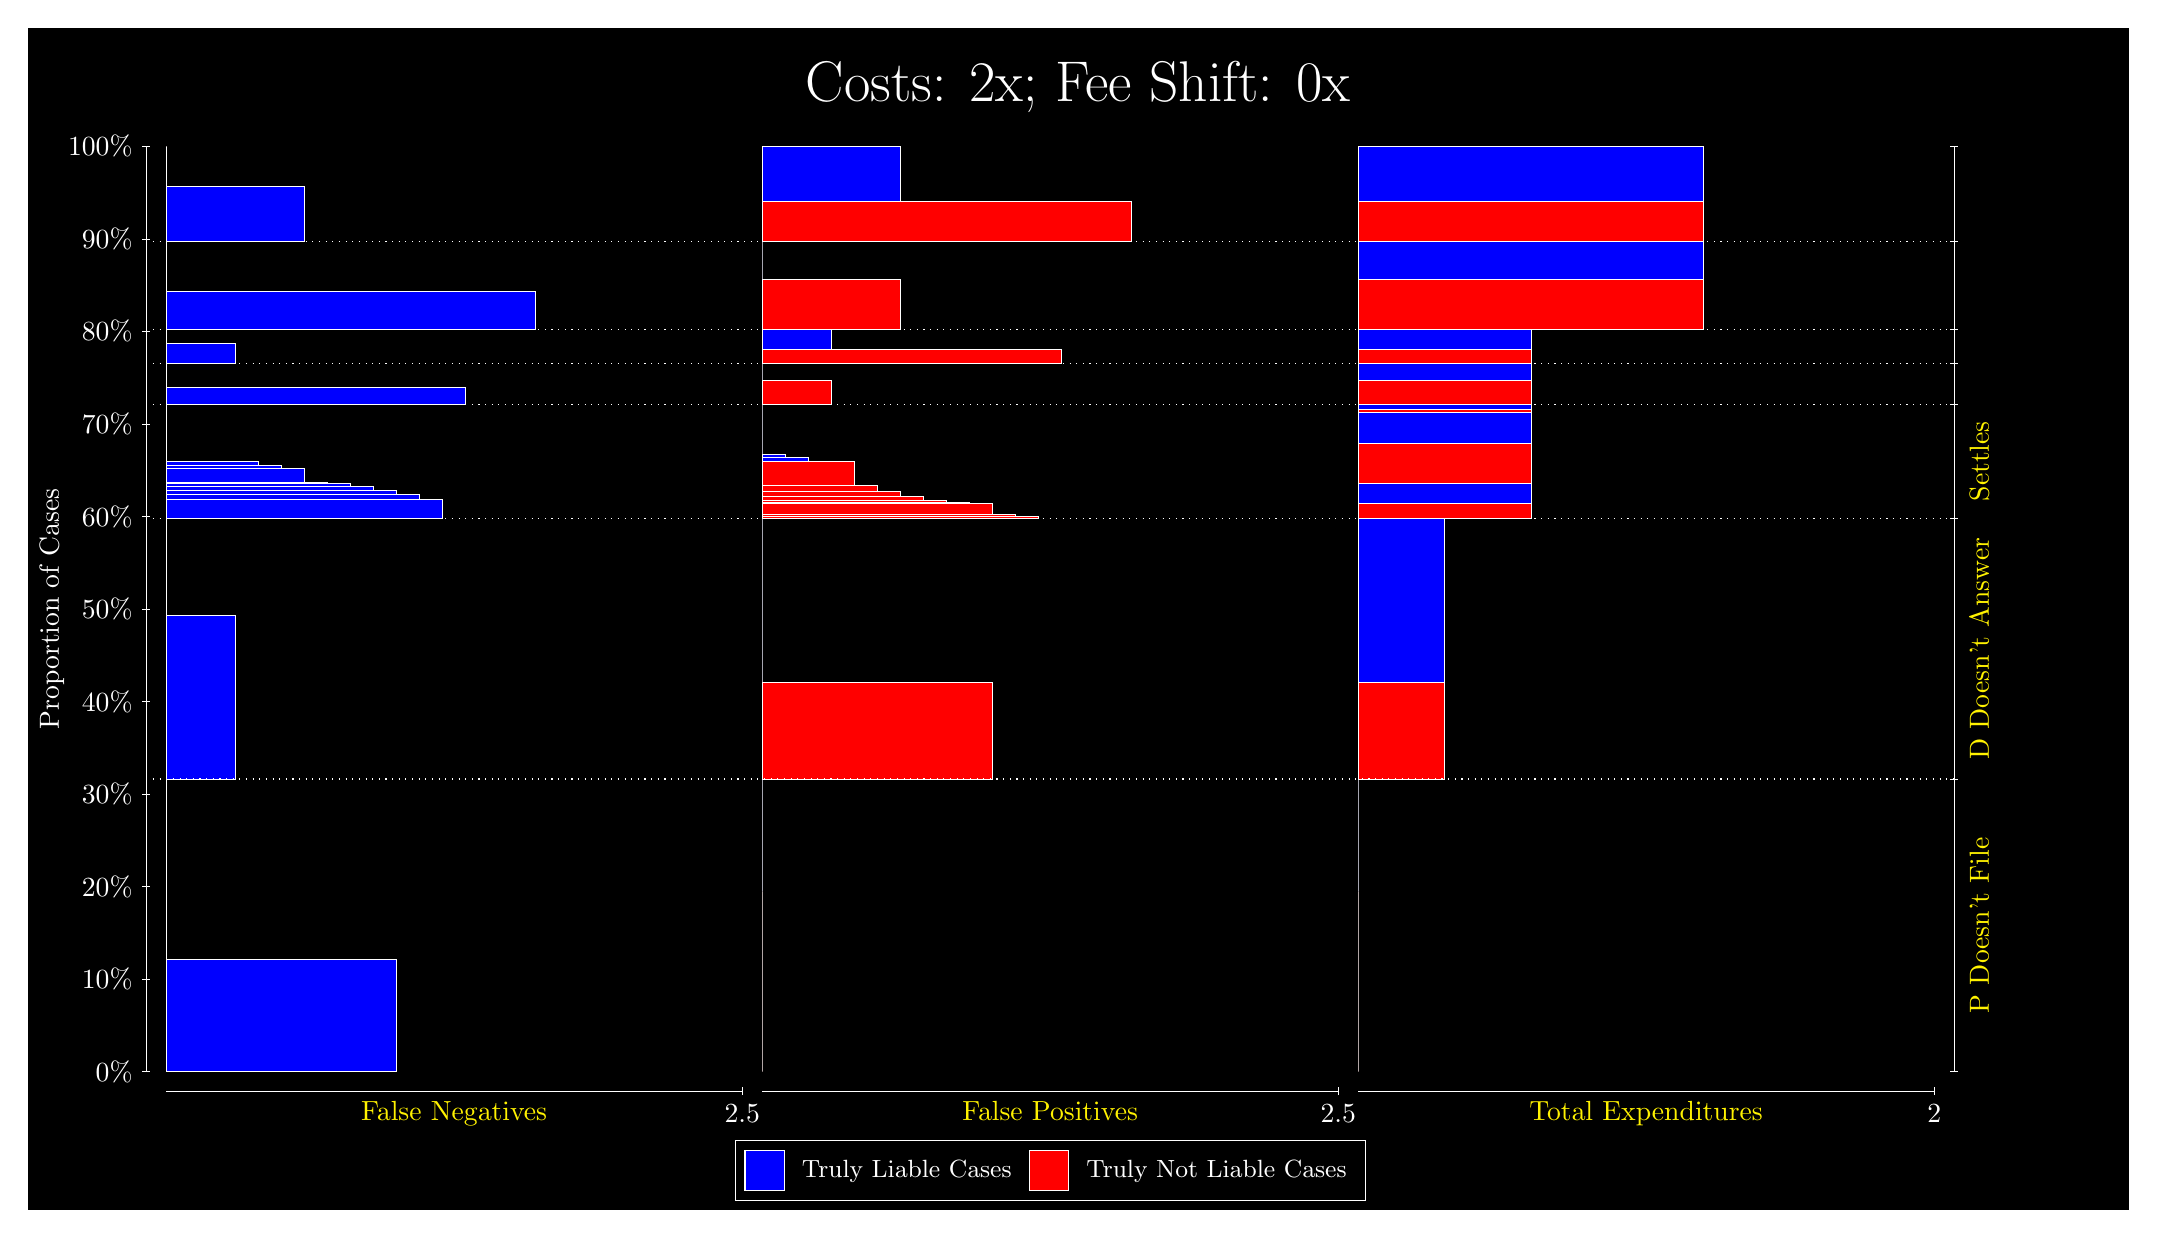
\begin{tikzpicture}
\draw[fill=black] (0,0) rectangle (26.667,15);
\draw[text=white] (0,13.5) rectangle (26.667,15) node[midway] {\huge Costs: 2x; Fee Shift: 0x};
\draw[white, very thin] (1.5,1.75) -- (1.5,13.5);
\node[rotate=90, text=white, anchor=center] at (0.3, 7.625) {Proportion of Cases};
\draw[white, very thin] (1.45,1.75) -- (1.55,1.75);
\node[text=white, anchor=east] at (1.45, 1.75) {0\%};
\draw[white, very thin] (1.45,2.925) -- (1.55,2.925);
\node[text=white, anchor=east] at (1.45, 2.925) {10\%};
\draw[white, very thin] (1.45,4.1) -- (1.55,4.1);
\node[text=white, anchor=east] at (1.45, 4.1) {20\%};
\draw[white, very thin] (1.45,5.275) -- (1.55,5.275);
\node[text=white, anchor=east] at (1.45, 5.275) {30\%};
\draw[white, very thin] (1.45,6.45) -- (1.55,6.45);
\node[text=white, anchor=east] at (1.45, 6.45) {40\%};
\draw[white, very thin] (1.45,7.625) -- (1.55,7.625);
\node[text=white, anchor=east] at (1.45, 7.625) {50\%};
\draw[white, very thin] (1.45,8.8) -- (1.55,8.8);
\node[text=white, anchor=east] at (1.45, 8.8) {60\%};
\draw[white, very thin] (1.45,9.975) -- (1.55,9.975);
\node[text=white, anchor=east] at (1.45, 9.975) {70\%};
\draw[white, very thin] (1.45,11.15) -- (1.55,11.15);
\node[text=white, anchor=east] at (1.45, 11.15) {80\%};
\draw[white, very thin] (1.45,12.325) -- (1.55,12.325);
\node[text=white, anchor=east] at (1.45, 12.325) {90\%};
\draw[white, very thin] (1.45,13.5) -- (1.55,13.5);
\node[text=white, anchor=east] at (1.45, 13.5) {100\%};

\draw[white, very thin] (24.457,1.75) -- (24.457,13.5);
\draw[white, very thin] (24.407,1.75) -- (24.507,1.75);
\node[anchor=west] at (24.407, 1.75) {};
\draw[white, very thin] (24.407,5.4651) -- (24.507,5.4651);
\node[anchor=west] at (24.407, 5.4651) {};
\draw[white, very thin] (24.407,8.777) -- (24.507,8.777);
\node[anchor=west] at (24.407, 8.777) {};
\draw[white, very thin] (24.407,10.225) -- (24.507,10.225);
\node[anchor=west] at (24.407, 10.225) {};
\draw[white, very thin] (24.407,10.746) -- (24.507,10.746);
\node[anchor=west] at (24.407, 10.746) {};
\draw[white, very thin] (24.407,11.173) -- (24.507,11.173);
\node[anchor=west] at (24.407, 11.173) {};
\draw[white, very thin] (24.407,12.293) -- (24.507,12.293);
\node[anchor=west] at (24.407, 12.293) {};
\draw[white, very thin] (24.407,13.5) -- (24.507,13.5);
\node[anchor=west] at (24.407, 13.5) {};

\draw[white, very thin, fill=blue] (1.75,1.75) rectangle (4.6775,3.177);
\draw[white, very thin, fill=red] (1.75,3.177) rectangle (1.75,5.4651);
\draw[white, very thin, fill=blue] (1.75,5.4651) rectangle (2.6283,7.5439);
\draw[white, very thin, fill=red] (1.75,7.5439) rectangle (1.75,8.777);
\draw[white, very thin, fill=blue] (1.75,8.777) rectangle (5.2631,9.0167);
\draw[white, very thin, fill=blue] (1.75,9.0167) rectangle (4.9703,9.0843);
\draw[white, very thin, fill=blue] (1.75,9.0843) rectangle (4.6775,9.1313);
\draw[white, very thin, fill=blue] (1.75,9.1313) rectangle (4.3848,9.1807);
\draw[white, very thin, fill=blue] (1.75,9.1807) rectangle (4.3848,9.1848);
\draw[white, very thin, fill=blue] (1.75,9.1848) rectangle (4.092,9.219);
\draw[white, very thin, fill=blue] (1.75,9.219) rectangle (3.7993,9.2308);
\draw[white, very thin, fill=blue] (1.75,9.2308) rectangle (3.5065,9.407);
\draw[white, very thin, fill=blue] (1.75,9.407) rectangle (3.2138,9.4525);
\draw[white, very thin, fill=blue] (1.75,9.4525) rectangle (2.921,9.4957);
\draw[white, very thin, fill=red] (1.75,9.4957) rectangle (1.75,10.225);
\draw[white, very thin, fill=blue] (1.75,10.225) rectangle (5.5558,10.443);
\draw[white, very thin, fill=red] (1.75,10.443) rectangle (1.75,10.746);
\draw[white, very thin, fill=blue] (1.75,10.746) rectangle (2.6283,11);
\draw[white, very thin, fill=red] (1.75,11) rectangle (1.75,11.173);
\draw[white, very thin, fill=blue] (1.75,11.173) rectangle (6.4341,11.655);
\draw[white, very thin, fill=red] (1.75,11.655) rectangle (1.75,12.293);
\draw[white, very thin, fill=blue] (1.75,12.293) rectangle (3.5065,12.989);
\draw[white, very thin, fill=red] (1.75,12.989) rectangle (1.75,13.5);
\draw[white, very thin, fill=red] (9.3189,1.75) rectangle (9.3189,4.0381);
\draw[white, very thin, fill=blue] (9.3189,4.0381) rectangle (9.3189,5.4651);
\draw[white, very thin, fill=red] (9.3189,5.4651) rectangle (12.246,6.6981);
\draw[white, very thin, fill=blue] (9.3189,6.6981) rectangle (9.3189,8.777);
\draw[white, very thin, fill=red] (9.3189,8.777) rectangle (12.832,8.8016);
\draw[white, very thin, fill=red] (9.3189,8.8016) rectangle (12.539,8.8297);
\draw[white, very thin, fill=red] (9.3189,8.8297) rectangle (12.246,8.9617);
\draw[white, very thin, fill=red] (9.3189,8.9617) rectangle (11.954,8.9736);
\draw[white, very thin, fill=red] (9.3189,8.9736) rectangle (11.661,9.0065);
\draw[white, very thin, fill=red] (9.3189,9.0065) rectangle (11.368,9.0573);
\draw[white, very thin, fill=red] (9.3189,9.0573) rectangle (11.075,9.1151);
\draw[white, very thin, fill=red] (9.3189,9.1151) rectangle (10.783,9.1958);
\draw[white, very thin, fill=red] (9.3189,9.1958) rectangle (10.49,9.5064);
\draw[white, very thin, fill=blue] (9.3189,9.5064) rectangle (9.9044,9.5495);
\draw[white, very thin, fill=blue] (9.3189,9.5495) rectangle (9.6116,9.5951);
\draw[white, very thin, fill=blue] (9.3189,9.5951) rectangle (9.3189,10.225);
\draw[white, very thin, fill=red] (9.3189,10.225) rectangle (10.197,10.528);
\draw[white, very thin, fill=blue] (9.3189,10.528) rectangle (9.3189,10.746);
\draw[white, very thin, fill=red] (9.3189,10.746) rectangle (13.125,10.918);
\draw[white, very thin, fill=blue] (9.3189,10.918) rectangle (10.197,11.173);
\draw[white, very thin, fill=red] (9.3189,11.173) rectangle (11.075,11.811);
\draw[white, very thin, fill=blue] (9.3189,11.811) rectangle (9.3189,12.293);
\draw[white, very thin, fill=red] (9.3189,12.293) rectangle (14.003,12.804);
\draw[white, very thin, fill=blue] (9.3189,12.804) rectangle (11.075,13.5);
\draw[white, very thin, fill=red] (16.888,1.75) rectangle (16.888,4.0381);
\draw[white, very thin, fill=blue] (16.888,4.0381) rectangle (16.888,5.4651);
\draw[white, very thin, fill=red] (16.888,5.4651) rectangle (17.986,6.6981);
\draw[white, very thin, fill=blue] (16.888,6.6981) rectangle (17.986,8.777);
\draw[white, very thin, fill=red] (16.888,8.777) rectangle (19.083,8.97);
\draw[white, very thin, fill=blue] (16.888,8.97) rectangle (19.083,9.226);
\draw[white, very thin, fill=red] (16.888,9.226) rectangle (19.083,9.7224);
\draw[white, very thin, fill=blue] (16.888,9.7224) rectangle (19.083,10.126);
\draw[white, very thin, fill=red] (16.888,10.126) rectangle (19.083,10.166);
\draw[white, very thin, fill=blue] (16.888,10.166) rectangle (19.083,10.225);
\draw[white, very thin, fill=red] (16.888,10.225) rectangle (19.083,10.528);
\draw[white, very thin, fill=blue] (16.888,10.528) rectangle (19.083,10.746);
\draw[white, very thin, fill=red] (16.888,10.746) rectangle (19.083,10.918);
\draw[white, very thin, fill=blue] (16.888,10.918) rectangle (19.083,11.173);
\draw[white, very thin, fill=red] (16.888,11.173) rectangle (21.279,11.811);
\draw[white, very thin, fill=blue] (16.888,11.811) rectangle (21.279,12.293);
\draw[white, very thin, fill=red] (16.888,12.293) rectangle (21.279,12.804);
\draw[white, very thin, fill=blue] (16.888,12.804) rectangle (21.279,13.5);
\draw[white, dotted] (1.5,5.4651) -- (24.457,5.4651);
\draw[white, dotted] (1.5,8.777) -- (24.457,8.777);
\draw[white, dotted] (1.5,10.225) -- (24.457,10.225);
\draw[white, dotted] (1.5,10.746) -- (24.457,10.746);
\draw[white, dotted] (1.5,11.173) -- (24.457,11.173);
\draw[white, dotted] (1.5,12.293) -- (24.457,12.293);
\draw[white, very thin] (1.75,1.5) -- (9.0689,1.5);
\node[text=yellow, anchor=north] at (5.4094, 1.5) {False Negatives};
\draw[white, very thin] (9.0689,1.45) -- (9.0689,1.55);
\node[text=white, anchor=north] at (9.0689, 1.45) {2.5};

\draw[white, very thin] (9.3189,1.5) -- (16.638,1.5);
\node[text=yellow, anchor=north] at (12.978, 1.5) {False Positives};
\draw[white, very thin] (16.638,1.45) -- (16.638,1.55);
\node[text=white, anchor=north] at (16.638, 1.45) {2.5};

\draw[white, very thin] (16.888,1.5) -- (24.207,1.5);
\node[text=yellow, anchor=north] at (20.547, 1.5) {Total Expenditures};
\draw[white, very thin] (24.207,1.45) -- (24.207,1.55);
\node[text=white, anchor=north] at (24.207, 1.45) {2};

\node[text=yellow, centered, rotate=90] at (24.777, 3.6075) {P Doesn't File};
\node[text=yellow, centered, rotate=90] at (24.777, 7.121) {D Doesn't Answer};
\node[text=yellow, centered, rotate=90] at (24.777, 9.501) {Settles};





\draw (12.978300999999998,1.5) node[draw=none] (baseCoordinate) {};
\begin{scope}[align=center]
        \matrix[scale=0.5, draw=white, below=0.5cm of baseCoordinate, nodes={draw}, column sep=0.1cm]{
            \node[rectangle, draw, minimum width=0.5cm, minimum height=0.5cm, fill=blue] {}; &
            \node[draw=none, font=\small, text=white] (B) {Truly Liable Cases}; &
            \node[rectangle, draw, minimum width=0.5cm, minimum height=0.5cm, fill=red] {}; &
            \node[draw=none, font=\small, text=white] (B) {Truly Not Liable Cases}; \\
            };
\end{scope}

\end{tikzpicture}
\end{document}